\subsubsection{Components under the Rate Reward}

\label{sec:rate_ablation}

We add five settings under the current transitions: remove graph features, remove rule features, remove the action mask, remove the training call penalty, or use a calibrated small count penalty. Ten seeds and 250 episodes per setting give fifty new models. The ten existing rate-DDQN checkpoints supply the matched complete-policy reference. All settings are evaluated on thirty further corruption seeds of the same base graph, giving 2,100 policy--seed--scenario outcomes including the heuristic. No model is selected by these outcomes.

The feature removals zero the specified observation entries during training and evaluation. Other observations and the action mask remain available. The no-mask setting selects from all eight actions in both behavior and target updates. Unavailable graph actions can be no-ops, and repeated rule acquisition can incur call cost; the underlying operators are unchanged. The no-call-cost setting removes only that training reward term. Evaluation uses the common rate reward.

\begin{table}[t]

\centering

\caption{Current-reward component study. Values average ten seed means, each over thirty common scenarios. Calls are simulated acquisition units; actual API requests are zero.}

\label{tab:rate_ablation}

\scriptsize

\begin{tabular}{lrrrr}

\toprule

Setting & F1 & Restoration & Calls & Unavailable \\

\midrule

Rate DDQN & 0.9952 & 0.9377 & 4.45 & 0.00 \\

No graph features & 0.9941 & 0.8938 & 4.10 & 0.00 \\

No rule features & 0.9775 & 0.6682 & 7.39 & 0.00 \\

No action mask & 0.9702 & 0.5776 & 6.23 & 8.26 \\

No call penalty & 0.9854 & 0.7686 & 5.54 & 0.00 \\

Small count penalty & 0.9905 & 0.9214 & 4.89 & 0.00 \\

Acquire-then-deficit & 0.9991 & 0.9884 & 4.00 & 0.00 \\

\bottomrule

\end{tabular}

\end{table}

Removing the mask lowers F1 by 2.50 points (95\% seed-bootstrap CI: $[-3.45,-1.62]$; Holm $p=0.0234$) and produces 8.26 unavailable selections per episode. It is the only contrast passing correction across twelve F1/restoration comparisons. Removing rule features also lowers mean F1 and raises acquisition cost, but its corrected test does not establish a stable effect across seeds. Every setting preserves initially correct reference facts in this controlled environment. The heuristic again has the highest mean F1 (99.91\%).

\paragraph{Penalty magnitude control.}

We calibrate a fixed count coefficient using twenty development rollouts with uniformly sampled feasible actions. The coefficient is the total rate burden divided by the total number of introduced violations: $\alpha=0.000164493$. This uses observed transitions, not reference facts or test outcomes. Small-count DDQN reaches 99.05\% F1, compared with 99.52\% for rate DDQN; the paired difference is $-0.47$ points (CI: $[-1.73,0.46]$, Holm $p=1$). At the base size, these results do not separate the benefit of rate normalization from a much smaller count coefficient.

\begin{figure*}[t]

\centering

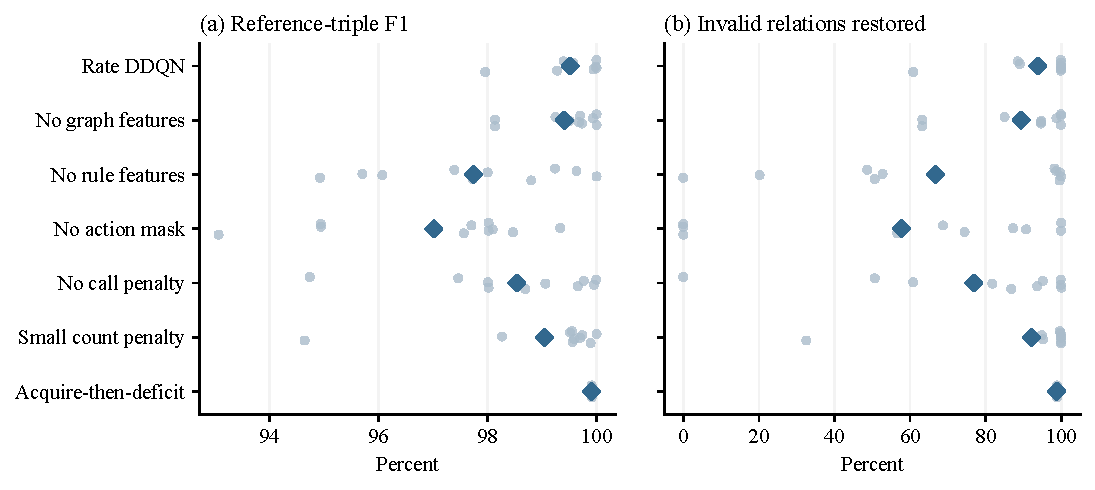
\includegraphics[width=0.93\textwidth]{figure/experiments/rate_ablation.pdf}

\caption{Current-reward ablations and the calibrated count control. Small dots show all ten training-seed means; diamonds show their average. Each seed mean uses thirty shared corruption scenarios. The heuristic is deterministic.}

\label{fig:rate_ablation}

\end{figure*}
